\documentclass[border=4pt]{standalone}
\usepackage{tikz}
\usetikzlibrary{positioning, arrows.meta, shapes.geometric, calc, fit, backgrounds}
\usepackage{amsmath,amssymb}
\begin{document}
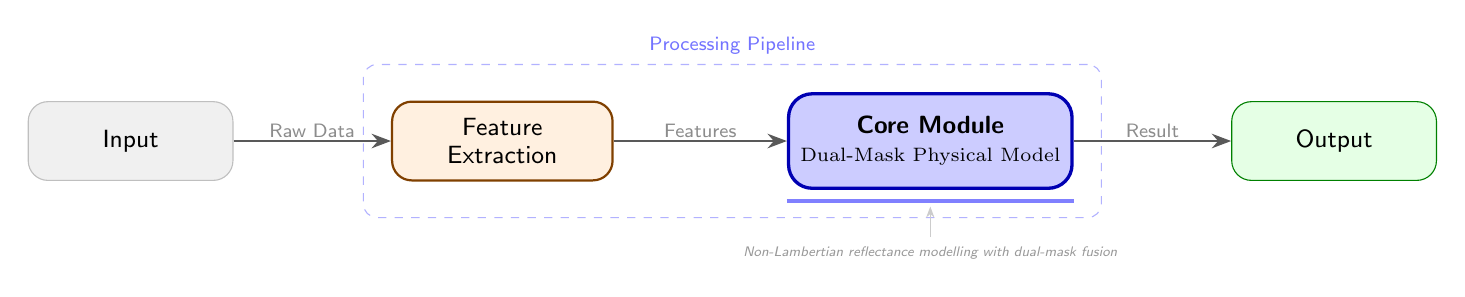
\begin{tikzpicture}[
  input/.style={draw, rounded corners=2.5mm, minimum width=2.6cm, minimum height=1.0cm,
                fill=gray!12, draw=gray!50, align=center,
                font=\sffamily\small},
  innov/.style={draw, rounded corners=3mm, minimum width=3.6cm, minimum height=1.2cm,
                fill=blue!20, draw=blue!70!black, line width=1.2pt, align=center,
                font=\sffamily\small\bfseries},
  proc/.style={draw, rounded corners=2.5mm, minimum width=2.8cm, minimum height=1.0cm,
               fill=orange!12, draw=orange!50!black, line width=0.8pt, align=center,
               font=\sffamily\small},
  output/.style={draw, rounded corners=2.5mm, minimum width=2.6cm, minimum height=1.0cm,
                 fill=green!10, draw=green!50!black, align=center,
                 font=\sffamily\small},
  arr/.style={-{Stealth[length=7pt]}, thick, color=black!65},
  lbl/.style={font=\sffamily\scriptsize, text=black!45, fill=white, inner sep=1pt},
]

% --- Nodes in data-flow order (left to right) ---
\node[input] (m1) {Input};

\node[proc, right=2.0cm of m1] (m2) {Feature\\[-1pt]Extraction};

\node[innov, right=2.2cm of m2] (m3) {Core Module\\[-1pt]{\normalfont\scriptsize Dual-Mask Physical Model}};

\node[output, right=2.0cm of m3] (m4) {Output};

% --- Main-flow arrows ---
\draw[arr] (m1) -- node[lbl, above] {Raw Data} (m2);
\draw[arr] (m2) -- node[lbl, above] {Features} (m3);
\draw[arr] (m3) -- node[lbl, above] {Result} (m4);

% --- Decorative underline for innovation module ---
\draw[blue!50, line width=1.8pt, rounded corners=1pt]
  ([yshift=-4pt]m3.south west) -- ([yshift=-4pt]m3.south east);

% --- Subtle grouping: processing pipeline ---
\begin{scope}[on background layer]
  \node[draw=blue!30, dashed, rounded corners=5pt, inner sep=10pt,
        fit=(m2)(m3),
        label={[font=\sffamily\scriptsize, text=blue!55]above:Processing Pipeline}] {};
\end{scope}

% --- Auxiliary annotation below Core Module ---
\node[font=\sffamily\tiny\itshape, text=black!40, below=0.6cm of m3]
  (anno) {Non-Lambertian reflectance modelling with dual-mask fusion};
\draw[-{Stealth[length=4pt]}, thin, color=gray!40] (anno.north) -- ([yshift=-6pt]m3.south);

\end{tikzpicture}
\end{document}